\documentclass[11pt,twocolumn,varwidth=true,a4paper,fleqn]{article}
\usepackage{fullpage}
\usepackage{url}
\usepackage[margin=1.1in]{geometry}
\usepackage{graphicx}
\usepackage{csvsimple}
\usepackage{varwidth}
\usepackage{array}
\usepackage{float}
\usepackage{amsmath}
\usepackage{pgfplotstable}
\usepackage{amsmath }
\usepackage[T1]{fontenc}
\usepackage[compact]{titlesec}
\usepackage{authblk}

\author[1]{Bernstein Ran}
\author[2]{Shafir Tal}
\author[3]{Tsachor Rachelle}
\author[4]{Studd Karen}
\author[1]{Schuster Assaf}
\affil[1]{Department of Computer Science, Technion I.I.T, Haifa, Israel}
\affil[2]{The Graduate School of Creative Arts Therapies, University of Haifa}
\affil[3]{School of Theatre \& Music, The University of Illinois at Chicago}
\affil[4]{School of Dance, George Mason University}

\begin{document}
\nocite{*}
\newcolumntype{M}{>{\begin{varwidth}{3cm}}l<{\end{varwidth}}}

\title{Laban Movement Analysis using Kinect}
\date{}
\maketitle
\begin{quote}{``Man moves in order to satisfy a need.`` ---\textup{Rudolph Laban}}
\end{quote}
\begin{abstract}
\textbf{Laban Movement Analysis (LMA) is a method for describing, interpreting
and documenting all varieties of human movement. 
Analyzing movements using LMA is advantageous over kinematic description, 
as it captures their qualitative aspects in addition to the quantitative. 
Thus, in recent years, LMA is increasingly becoming the preferred method for movement analysis. 
In this study we developed a Machine Learning (ML) method for recognizing Laban qualities from 
a markerless Motion Capture (MOCAP) camera --- Microsoft's Kinect. 
We believe that we are the first succeeded identifying LMA with a ubiquitous
sensor.
There no papers similar enough to ours for a performance comparison,
but our work obtained a recall and precision rate of about 60\%  averaged over
the qualities, result that is a solid foundation for a future work, and even a
success by itself.}
\end{abstract}
\section{Introduction}
Our goal is to create a method for automated identification of Laban qualities that 
characterize any movement sequence, using Kinect. 
Our problem presents three challenges. The first is
quantifying subtle qualities for which a well-defined quantification has not yet been found. 
The second challenge is handling noisy sensory data with an in-home setup, and the
third is keeping our method as general as possible --- We are developing a system capable of 
handling different scenarios (dancing and acting, for example), and different postures 
(sitting and standing, for example), by different people of different backgrounds (if any) 
in movement. 
\\\\We propose a low-cost (100\$), non-intrusive
(markerless), ubiquitous (76 million sensors around the world) system that can recognize Laban qualities using the Kinect sensor and Software Development Kit (SDK).
For evaluation, we have created our own dataset and applied several ML
techniques on it, in several learning settings. We chose to use ML (instead of rule based algorithms), so 
we would be able to use all of the rich data provided by the Kinect sensor rather than focus on a very 
subtle feature extraction method that requires domain expertise. Using ML gave us
an opportunity to reverse engineer the learned models and learn about
our problem's intrinsic characteristics, such as which features are predictive
of which qualities. The system obtained a recall and precision rate of between
40-60\% in the more subtle qualities, and 60-90\% in the more expressive ones.
\subsection{Motivation for Automated LMA}
There are numerous applications for computerized identification of the qualities that characterize each possible human movement. Examples include the generation and control of specific expressive movements 
of avatars, virtual characters, or robots in mixed reality scenarios
\cite{Masuda}; detection of personality traits during a job interview
\cite{levy2003use}; early detection, severity assessment or revealing of genetic tendency (phenotype) towards various illnesses such as Alzheimer's,
autism, Parkinson's disease \cite{camurri2003application}, or schizophrenia,
based on analysis of the person's motor behavior. Automated emotion recognition from movement is another 
important application, which may have a variety of uses such as online feedback 
to presenters to help them convey through their body language the emotional message they want to communicate 
(e.g., politicians and public speakers or actors in training) \cite{nguyen2012online}; or recognition 
of people's emotions during interactive games such as those played using the Xbox \cite{Zacharatos}. 
\\\\For reducing our data collection and analysis effort, we focused our work on 18 Laban qualities (as listed in table \ref{mixedSummary}) that have been found predictive for emotional state \cite{ShafirPrivate}.

\subsection{Laban movement analysis}
LMA is a formal language for motion description first developed by Rudolf Laban \cite{Laban} and colleagues in the middle of the 20th century. 
LMA describes both conscious and unconscious human movement, based on Laban's categories of \textit{Body}, \textit{Effort}, \textit{Shape}, and \textit{Space}. 
LMA has been used in the fields of dance, acting, athletics, physical therapy, and psychology and behavioral science.
LMA helps actors create momentary moods and portray personality traits through
movement. For example, LMA work investigates the \textit{Effort} properties
\textit{Flow}, \textit{Space}, \textit{Time} and \textit{Weight} of all movement and helps actors 
think specifically about why their character might move in a jerky, fast, light and direct manner 
versus a heavy, slow, indirect and uninterrupted manner.
\begin{figure*}[ht]
\centering
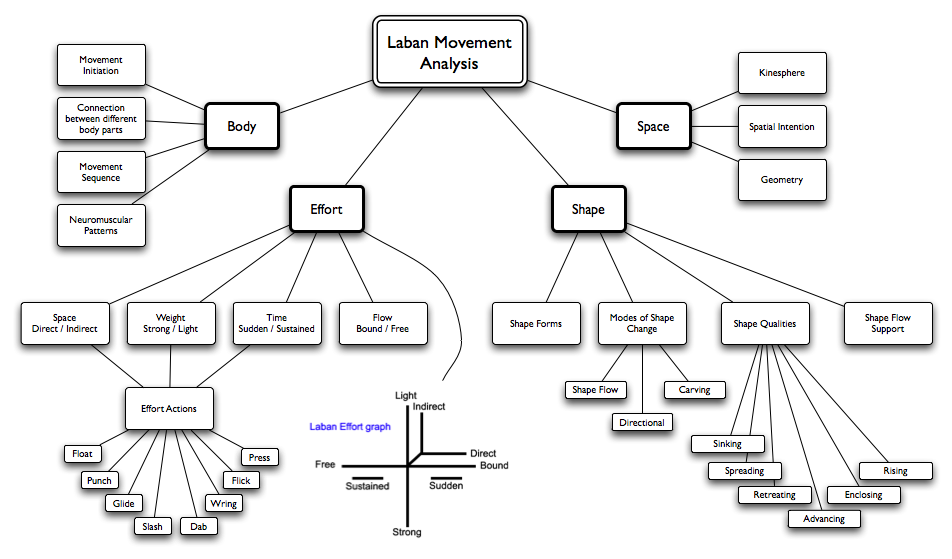
\includegraphics[width=\textwidth]{laban.png}
\caption{Main axes of LMA. Taken from \cite{labanTree}}
\label{labanTree}
\end{figure*}
The entire LMA hierarchy is shown in figure \ref{labanTree}.

\subsection{Kinect Sensor Data}
Figure \ref{skeleton} shows the skeleton provided by Kinect's SDK. 
\begin{figure}[h]
\centering
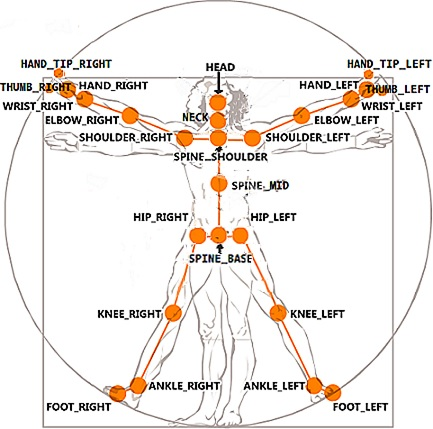
\includegraphics[width=60mm]{skeleton.jpg}
\caption{Skeleton positions relative to the human body}
\label{skeleton}
\end{figure}
Once the skeleton is detected, the 3D coordinates of all the joints of the
user's body --- with the exception of joints that are not visible (e.g., a user's
hand is behind his or her back) --- are provided.
As seen in Figure \ref{Coordinate}, the coordinates are in a ``real-world''
coordinate system, whose origin [0,0,0] is in the sensor and whose x-, y-, and
z-axis are as depicted below.
\begin{figure}[h]
\centering
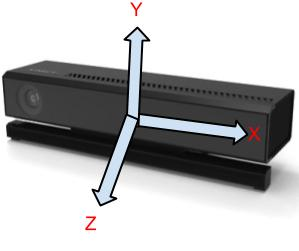
\includegraphics[width=60mm]{KinectV2CoordinateSystem.jpg}
\caption{Kinect Coordinate System}
\label{Coordinate}
\end{figure}

\subsection{Related Work}
Several attempts were made to recognize Laban qualities. The first was Chi et al. \cite{chi2000emote}, who quantified \textit{Effort} and \textit{Shape} for animation. Most of the other attempts were for emotion recognition in the context of Human Robot Interaction (HRI). Martin et al. \cite{martin} analyzed the importance of gestures in emotion recognition for HRI. Masuda et al. generated emotional body motion for a human 
form robot \cite{Masuda}. Rett et al. proposed a human motion recognition 
system using a Bayesian reasoning framework \cite{Rett}. The second line of works focused on LMA (not on emotions), but not using Kinect. Lourens et al. \cite{lourens2010communicating} used video data and Samadani et al.
\cite{samadani2013laban} used a high quality MOCAP camera, but both of them
analyzed only hand gestures. A third line of works used Kinect as the main
sensor for skeletal information. Gabel et al.
\cite{gabel2012full} used Kinect for gait analysis. The work of
Zacharatos et al. \cite{Zacharatos} was inspired by LMA for emotion recognition using Kinect. His feature extraction method was influenced by LMA principles, but he did not attempt to recognize the qualities themselves. Kim et al. \cite{kim} did attempt to do so but not on a real dataset and their work did not include a performance evaluation.
\section{Method}
Because we are the first to handle Laban recognition with
Kinect, we had to create a dataset from scratch. To reduce the noise, and ensure that we capture the essence of the Laban qualities in our dataset, we decided that most of it should be built by recording several Certified [Laban] Movement Analysts (CMA), with just a few validation clips taken from recordings of ordinary people. We did not want to constrain the lengths of the clips to be equal, so in order to get feature vectors of uniform length (regardless of the original length of the clips),
every feature is function of a whole clip (for example, the variability of the
elbow's acceleration). On the uniform length feature vector we applied feature
selection, single task learning (learning a model for every quality separately),
and multitask learning (learning a model for all the qualities together).
\subsection{Clip Collection}
Two main datasets were collected: 
\begin{itemize}
  	\item 
	 CMA dataset - includes 6 CMAs performing in about
	80 clips each (a total of 550 clips). Every clip is about 3 seconds long, and the CMAs executed combinations of the 18 qualities. 
	To achieve uniform distribution of the Laban qualities over the dataset, in every 
	clip the CMA was asked to perform actions that include several specific qualities, 
	and nothing but them.
	
	\begin{figure}[h]
	\centering
	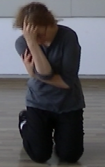
\includegraphics[width=30mm]{Rachelle.png}
	\caption{CMA during a clip}
	\label{Rachelle}
	\end{figure}
	
	\item 
	Non-CMA dataset - includes 2 subjects without a background in movement
	analysis, performing 30 clips each. Every clip is also about 3 seconds long,
	and the subject was asked to perform one out of several
	tasks.
\end{itemize}
\subsection{Clip Labeling}
To achieve a ground truth labeling for the two datasets, every clip was tagged by
a committee of 2 CMAs who determined which Laban qualities appear in the
clip. The use of a committee decision instead of the subjective opinion of one
CMA decreases the labeling noise and the decision is considered as ground truth.
\subsection{Feature Extraction}
Due to the unequal length of clips, all the extracted features are in whole clip 
granularity. We extracted two groups of features, the first is a relatively
small, and contains about 100 features that each one of them is designed for a
specific quality. The second group contains about 6000 features, and exploits the rich data that
is provided by Kinect, by extracting from every joint in the skeleton, the
angular velocity, acceleration, and jerk. For every joint/metric pair, the mean,
variance, skew, and kurtosis were extracted (the extraction of the last four moments is denoted as $\phi$).
\\\\We denote $\vec{P}_{j}(t)$ as the vector (as we get it from the Kinect) of
the position of joint $j$ in time $t$ in a clip with $n$ frames, and
$\alpha_{j}$ is a coefficient proportional to the mass around the joint.
\subsubsection{Shape Analysis: Sagittal Plane}
Laban shape analysis of the sagittal plane is based on the distinction
between two qualities, \textit{Advance} and \textit{Retreat}. This distinction was quantified by projecting the 
velocity vector of the Center of Mass (CM) on the vector of the front of the
body.
The CM was approximated in this case by the average of all the joints. 
The front of the body was approximated by the perpendicular vector to the vector 
between the Left Shoulder (LS) and
the Right Shoulder (RS).
\\\\If $sag$ stands for sagittal, then from the definition of CM of a physical
system,
\\
\\$\vec{P}_{CM}(t) = \sum_{j \in Joints} \alpha_{j}\vec{P}_{j}(t),
\\
\\\vec{P}_{shoulders}(t)=\vec{P}_{LS}(t)-\vec{P}_{RS}(t),$
\\\\the front is perpendicular to $\vec{P}_{shoulders}$, so we can easily calculate it with:
\\\[\vec{P}_{front}=\vec{P}_{shoulders}\left( \begin{array}{ccc}
0 & 0 & 1 \\
0 & 1 & 0 \\
-1 & 0 & 0 \end{array} \right),\]
\\\\$S_{sag}(t) = \vec{P}_{CM}(t)\cdot\vec{P}_{front}(t),$ 
\\\\$\vec{F}_{sag} = \phi([S_{sag}(1), \ldots S_{sag}(n)]),$
\\\\where $\phi$ was denoted in the beginning of the section.
\subsubsection{Shape Analysis: Horizontal Axis}
Here the distinction is between \textit{Spreading} and \textit{Enclosing} on the horizontal axis.
This distinction was quantified by measuring the average distance between every joint to 
the vertical axis of the body that extends from the Head (H) to the Spine Base (SB).
\\
\\$d_{j} = \frac{\left|(\vec{P}_{j}-\vec{P}_{SB})\times
(\vec{P}_{j}-\vec{P}_{H})\right|}{\left|\vec{P}_{H}-\vec{P}_{SB}\right|},
\\
\\S_{horiz}(t) = \sum_{j \in Joints} d_{j}(t),
\\
\\\vec{F}_{horiz} = \phi([S_{horiz}(1), \ldots S_{horiz}(n)]),$
\subsubsection{Shape Analysis: Vertical Axis}
Here the distinction is between \textit{Rise} and \textit{Sink} on the vertical
axis.
This distinction was quantified by measuring the average distance on axis y of each joint from the CM. This quantification is based on the assumption that the body
is ``longer'' when rising.
\\\\$S_{vert}(t) = \sum_{j \in Joints}
\left|\vec{P}_{j}-\vec{P}_{CM}\right|,
\\\\\vec{F}_{vert} = \phi([S_{vert}(1), \ldots S_{vert}(n)]),$
\subsubsection{LMA Effort Analysis: Time Category}
Here the distinction is between \textit{Sudden} and \textit{Sustained}. This quality was quantified by the skew of the acceleration, relying on the assumption that the
acceleration of a sudden movement will be skewed further to the left, i.e., will get
a higher value at the beginning of the movement.
\subsubsection{Effort Analysis: Space Category}
Here the distinction is between \textit{direct} and \textit{Indirect} motion.
This quality was quantified by the angle between the movement vector of a joint to the next one,
relying on the assumption that in direct movement every vector will be in
the same direction as the last (the angle between them is small).
The velocity direction $V$ is calculated by
$\vec{V}_{j}(t) = \vec{P}_{j}(t+1) - \vec{P}_{j}(t),$
and the angles between a direction to the next one is calculated with the inner product
$\vec{A}_{j}(t) = \vec{V}_{j}(t+1) \cdot \vec{V}_{j}(t).$

\subsection{Performance Evaluation}
From a statistical point of view, we have 18 possible labels (Laban qualities) for every clip. 
Each clip was a combination of just a few of these, often 3-4, which means that there is about 
an 85\% chance that a quality won't appear in a clip. Due to this sparsity, accuracy alone is 
not a relevant metric for the performance evaluation because one can get 85\% accuracy by stating 
that for every recording none of the qualities appear. 
A better evaluation would have to combine the precision and recall rates of the classifier. 
This can be done using the F1 score:
\begin{equation*}
F_{1} = \frac{2\cdot precision\cdot recall}{precision+recall}.
\end{equation*} 
\subsection{Feature Selection}
Every clip is extracted into a vector of 6120 features, most of which are noisy or redundant, thus requiring massive feature selection. The feature selection is done in three stages:
	\begin{itemize}
		\item
		Computing the Anova F-value for every feature over the training set. Cross-validation was used to determine the optimal number of features that should be
		left. As seen in Figure  \ref{selection}, filtering out most of the features yielded better          results than not filtering them, where using the top 4\% of features was optimal.
		\begin{figure}[ht!]
			\centering
			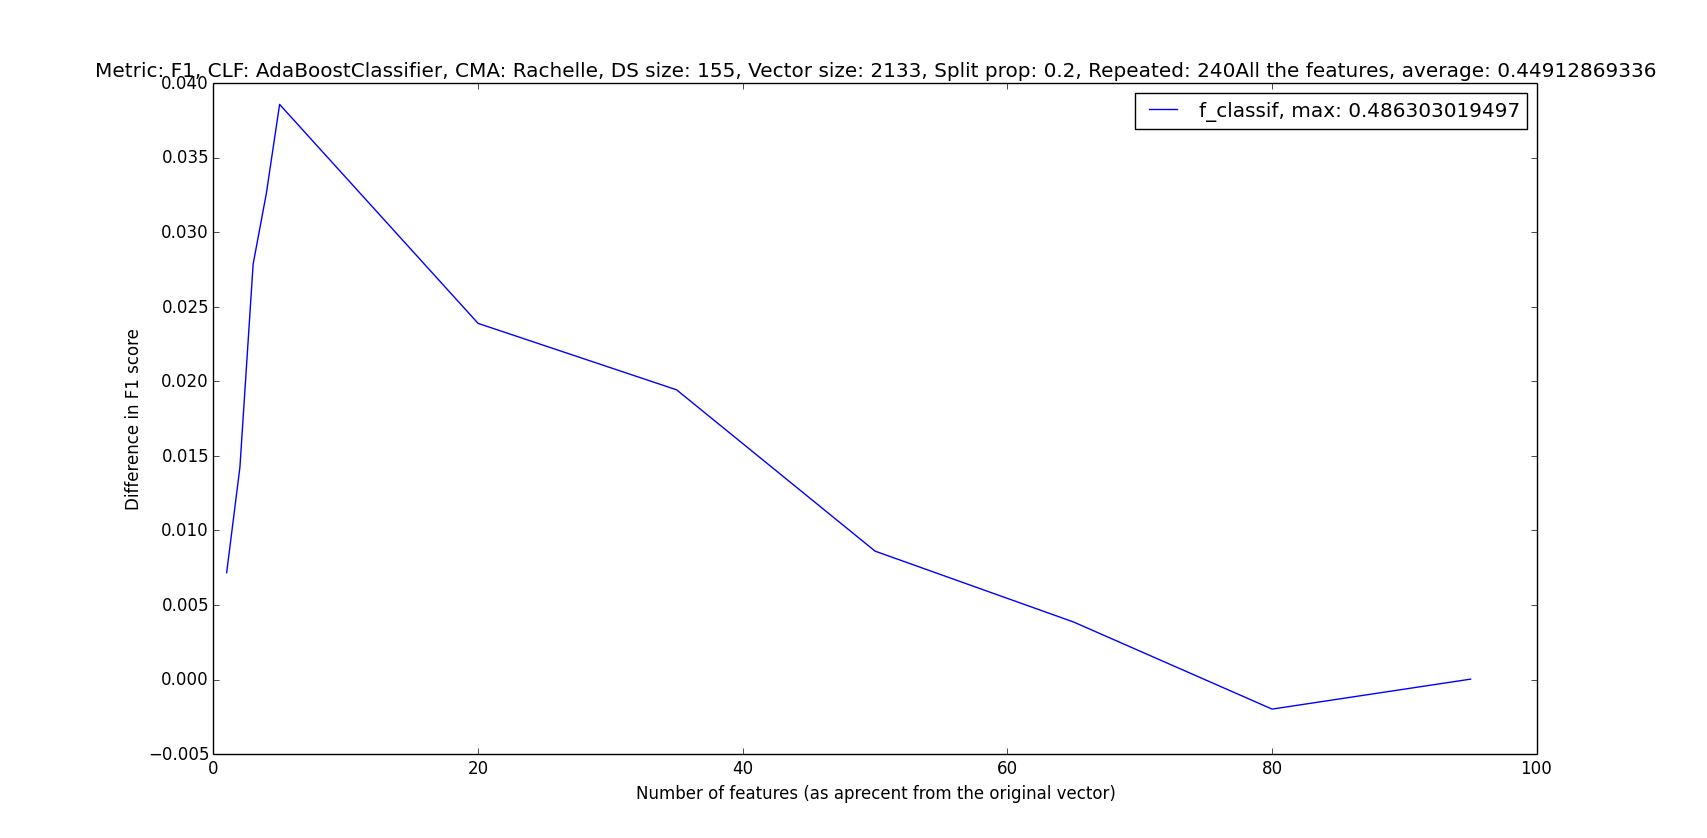
\includegraphics[width=60mm]{featureSelection.png}
			\caption{Influence of the number of features on the performance. The
			selection was made according to statistical significance.
			The blue line is the difference between the score with and without feature
			selection. It can be seen that the optimal fraction of features to select is
			4\%.}
			\label{selection}
			\end{figure}
		\item
			The second phase of feature selection was conducted by Information Gain (IG) rating of the features. As seen in Figure  \ref{igFromFclassif}, the optimal ratio was obtained by selecting the top 60\% out of the features that remained after the first
			phase of feature selection.
			 \begin{figure}[h]
				\centering
				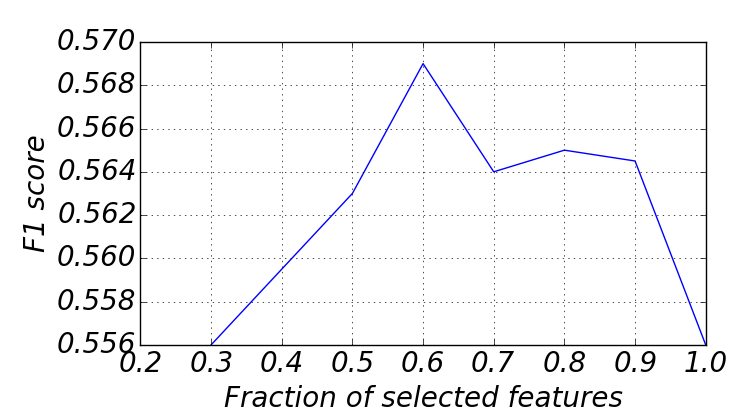
\includegraphics[width=60mm]{igFromFclassif.png}
				\caption{Influence of the number of features selected with IG from the subset
				of features chosen in the first phase on the performance. The
				optimal ratio was 60\%.}
				\label{igFromFclassif}
			\end{figure}
			Examples of qualities and their most significant feature are given in 
			Table \ref{bestFeatures}. The ``Information Gain'' metric used
			in the table is defined as:
			\begin{equation*}
			       IG(T,f) = H(T) - H(T|f),
			\end{equation*}
			where T is the training set, f is a feature, and H() is the information
			entropy of a dataset.
			 \begin{table*}
			   \centering
			   \csvautotabular{rankFeatures.csv}
			   \caption{Example of several qualities and the feature found to be
			   the most informative for them. ``Relative position'' stands for the
			   position of the joint relative to the ancestor joint in the joint
			   hierarchy.}
			   \label{bestFeatures}
			\end{table*}
		\item
		The third phase of feature section was conducted using the Least Absolute Shrinkage and
		Selection Operator (LASSO) regularization.
	\end{itemize}

\section{Experimental Setups and Results}
\subsection{Multilabel Classification}
Multilabel learning deals with the problem where each instance is associated
with multiple labels simultaneously, where the number of labels is not fixed
from instance to instance. The task of this learning paradigm is to predict
the label (Laban quality) set for each unseen instance (skeletal recording), 
by analyzing training instances with known label sets. The multilabel
approach taken in this paper is to break the LMA problem into 18
binary classification tasks --- one for every Laban quality --- where every binary
decision is whether or not the quality exists.
\\The following subsections will describe several experimental setups
where the results in each will serve as a baseline for the next.
\subsection{Per CMA Evaluation}
	In this experiment the train and test datasets are taken from the same
	CMA. The performance on every Laban quality separately 	is demonstrated on 
	a dataset of one of the CMAs in Figure \ref{oneCMAFinal}.
	In Figure \ref{oneCMASummary} the incremental evolution of the algorithm is 
	described from step to step with the next notation:
	\begin{itemize}
	\item 
	\textit{Chance} stands for randomly tossing a balanced coin in every
	classification decision.
	\item 
	\textit{NN} stands for applying the Nearest Neighbors algorithm.
	\item 
	\textit{LinearSVC} stands for Support Vector Classifier (SVC) with a linear
	kernel.
	\item 
	\textit{LabelBalancing} stands for giving greater weight to clips that
	contain the quality due to the small fraction of them in the whole
	dataset.
	\item 
	\textit{Lasso}, \textit{SFS} (Statistical Feature Selection), and \textit{InfoGain} 
	(information gain based feature selection) were described in the
	\textit{Feature Selection} section.
	\end{itemize}

\pgfplotstableread{
x         y    y-max  y-min
Chance          0.23 0.005 0.005
NN              0.26 0.025 0.025
LinearSVC       0.37 0.02  0.02
LabelBalancing  0.41 0.025 0.025
Lasso           0.44 0.025 0.025
SFS             0.48 0.045 0.045
InfoGain        0.53 0.045 0.045
}{\mytable}

\begin{figure}[ht]
\centering   
\begin{tikzpicture}
\begin{axis} [
    width=5cm,
    ymin=0.2,
    ylabel={F1 score},
    symbolic x coords={Chance,NN,LinearSVC,LabelBalancing,Lasso,SFS,InfoGain},
    xtick=data,
    x tick label style={rotate=90,anchor=east}
]
\addplot [ybar, fill=blue!50] 
  plot [error bars/.cd, y dir=both, y explicit]
  table [y error plus=y-max, y error minus=y-min] {\mytable};
\end{axis} 
\end{tikzpicture}
\caption{Evaluation of every CMA's dataset separately in the single task learning
		setting. Each column represents an additional step in the algorithm's evolution.
		The results are the average F1 score and its standard deviation (STD) between the CMAs.}
\label{oneCMASummary}
\end{figure}

\begin{figure*}
	\centering
	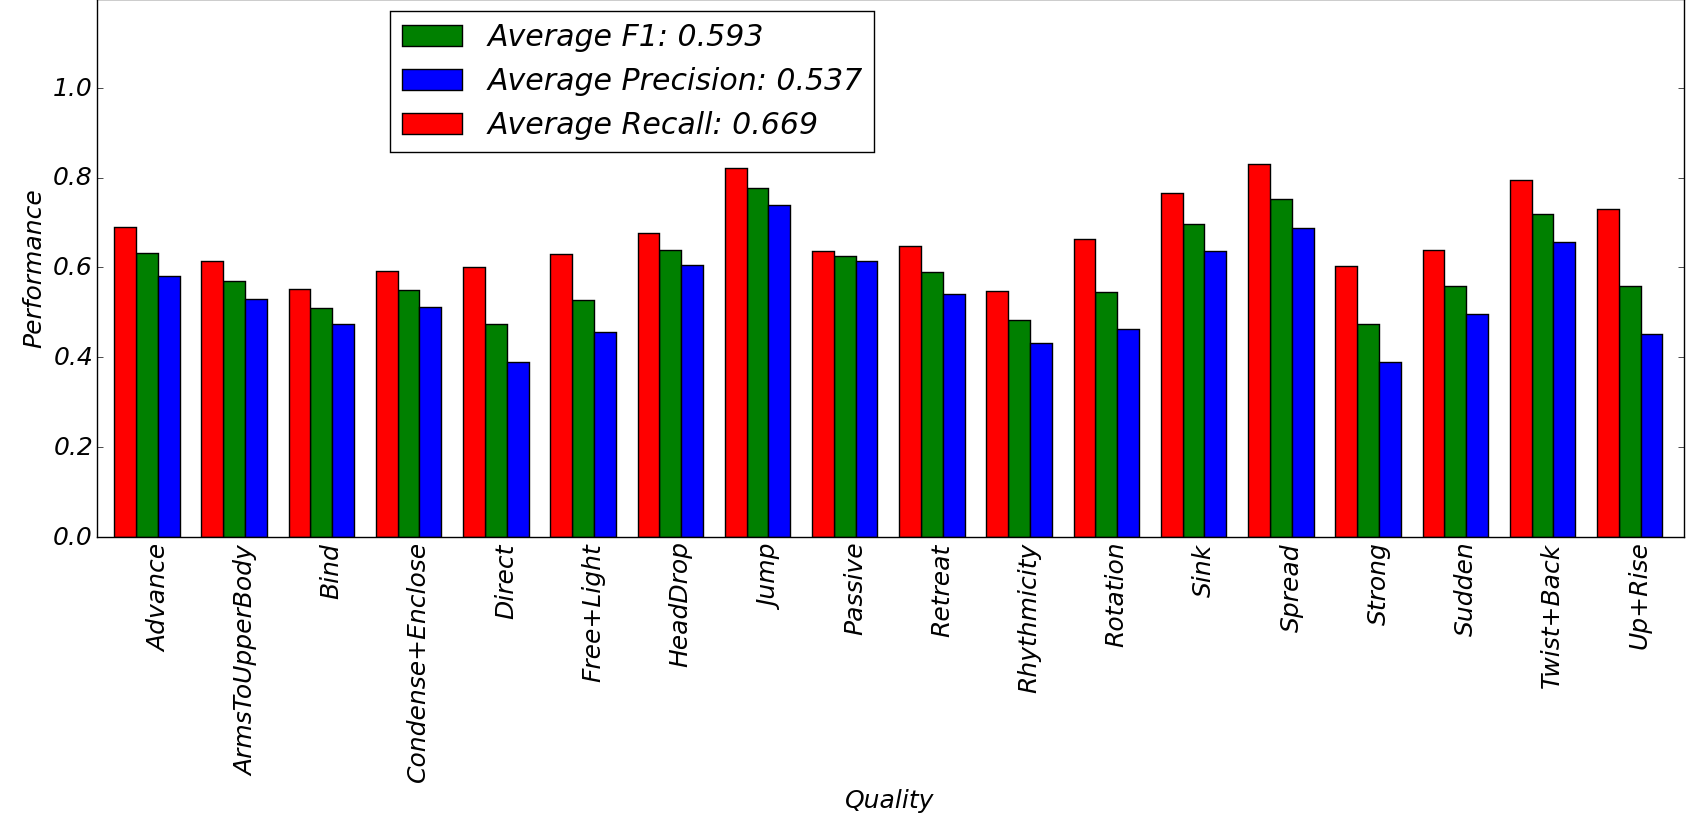
\includegraphics[width=\textwidth, height=60mm]{oneCMAFinalWithoutTitle.png}
	\caption{Recall, precision and F1 score of each Laban quality separately. The
	evaluation was conducted on a dataset that was captured on only one CMA.}
	\label{oneCMAFinal}
\end{figure*}
	
\subsection{Mixed Dataset Evaluation}
	In this section the datasets of all of the CMAs were mixed. In the learning
	and testing process the origin (CMA) of the instance was ignored. 
\subsubsection{Single Task Learning as a Baseline}
As a baseline we applied the SVC based flow that was described in the last
section on the mixed dataset. The results are shown in Figure \ref{mixedCMASummary}.
It can be seen that the performance improves in comparison to the
per CMA evaluation of the last section. There are two reasons for this
improvement, the first is the increase in the dataset's size when merging a few
CMA datasets together, and the second is diversity of the clips, which improves
the model's generalization ability.


\begin{figure}[ht!]
\centering
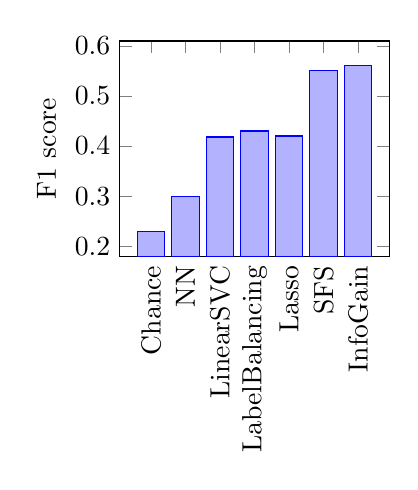
\begin{tikzpicture}
\begin{axis}[
    width=5cm,
    ybar stacked,
    enlargelimits=0.15,
    ylabel={F1 score},
    symbolic x coords={Chance,NN,LinearSVC,LabelBalancing,Lasso,SFS,InfoGain},
    xtick=data,
    x tick label style={rotate=90,anchor=east},
    ]
\addplot+[ybar] plot coordinates  {(Chance,0.23) (NN,0.3) (LinearSVC,0.418) 
		(LabelBalancing,0.43) (Lasso,0.42) (SFS, 0.55) (InfoGain,0.56)};

\end{axis}
\end{tikzpicture}
\caption{Evaluation on CMA mixture dataset in single task learning
		setting. Every Column is an additional step in the algorithm's evolution.}
\label{mixedCMASummary}
\end{figure}


\subsubsection{Multitask vs Single Task Learning}
We found that multitask learning for all the 18 qualities together exhibited superior 
performance to learning a classifier for each problem separately. For the
multitask setting we used Multitask Elastic Net (MEN) regularization, which is
the multitask regularization method of Zou et al. \cite{Zou}, where the
optimization objective is:
\\
\begin{equation}\label{eq:MEN}
	\|Y - XW\|^2_F+\lambda_1\cdot\|W\|_{2,1}+\lambda_2\cdot\|W\|^2_F,
\end{equation}    
  
$\lambda_1$, and $\lambda_2$ are hyper-parameters, where,
\\
\begin{equation*}
        \|W\|_{2,1} = \sum_i \sqrt{\sum_j w_{ij}^2},
\end{equation*} 
    i.e., the sum of norm of each row (also known as mixed norm), and 
\begin{equation*}
        \|W\|^2_F = \sum_i{\sum_j w_{ij}^2},
\end{equation*}     
	i.e., the Frobenius norm. 
Feature selection was carried out by averaging the statistical significance of
each feature with respect to all of the tasks (this is in contrast to the single
task learning flow, where every task had its own feature selection). As seen in
Table \ref{MultitaskVsSeparated}, the multitask setting improved the F score by
7\%, indicating that the tasks are correlated and more might be learned
from the small dataset when using this setting.	
 	\begin{table}[ht]
	  	\centering
		\begin{tabular}{|p{1.8cm}|p{1.8cm}|p{1.8cm}|}
		\hline
		Metric&Single task&Multitask\\\hline
		Precision&0.46&\textbf{0.59}\\\hline
		Recall&\textbf{0.71}&0.65\\\hline
		F1&0.56&\textbf{0.6}\\\hline
		\end{tabular}
		\caption{Multitask vs Single task learning performance evaluation on a CMA mixture
		dataset.}
	   \label{MultitaskVsSeparated}
	\end{table}

\subsubsection{Performance of Every Quality in Multitask Setting}
The performance over every quality as classified by the MEN in Table
\ref{mixedSummary}. During the MEN optimization ~\eqref{eq:MEN}, the mixed norm 
term $\|W\|_{2,1}$  promotes sparsity in the weights matrix $W$ such that for 
every row in the matrix, if one coordinate is equal to zero, then every coordinate 
in the row will be equal to zero.
\\The generalization ability of the model was enhanced by the fact that the
decision which features to select is influenced by all the qualities, (feature $f_i$ is 
selected in the MEN if the row $r_i$ in $W$ is not all zeros). The most
significant improvement were in the qualities that performed worse in the
single task learning setting (\textit{Strong} and \textit{Sudden} for example).
\begin{table}[!h]
	  	\centering
		\begin{tabular}{|p{3cm}|p{0.9cm}|p{0.9cm}|p{0.9cm}|}
		\hline
		Quality&Precis-ion&Recall&F1 score\\\hline
		Jump&0.89&0.81&0.85\\\hline
		Twist and Back&0.69&0.85&0.76\\\hline
		Sink&0.62&0.79&0.69\\\hline
		Rhythmicity&0.59&0.72&0.65\\\hline
		Spread&0.55&0.76&0.64\\\hline
		Head drop&0.60&0.66&0.63\\\hline
		Rotation&0.66&0.60&0.63\\\hline
		Free and Light&0.45&0.94&0.61\\\hline
		Up and Rise&0.67&0.54&0.60\\\hline
		Condense and Enclose&0.44&0.84&0.58\\\hline
		Arms To Upper Body&0.67&0.54&0.60\\\hline
		Advance&1.00&0.38&0.55\\\hline
		Retreat&0.50&0.59&0.54\\\hline
		Passive&0.40&0.85&0.54\\\hline
		Bind&0.44&0.61&0.51\\\hline
		Direct&0.56&0.49&0.52\\\hline
		Sudden&0.61&0.41&0.49\\\hline
		Strong&0.29&0.42&0.34\\\hline
		\textbf{Average}&\textbf{0.59}&\textbf{0.65}&\textbf{0.60}\\\hline
		\textbf{SD}&\textbf{0.17}&\textbf{0.17}&\textbf{0.11}\\\hline
		\end{tabular}
		\caption{Recall, precision and F1 score of each Laban quality on a CMA
		   mixture dataset. The learning was done in a multitask setting. The number of
		   features that weren't nullified by the mixed norm regularization is
		   282 (same features for all of the tasks). The F1 average and standard
		   deviation over the qualities is shown in the last row of the table.}
	   \label{mixedSummary}
	\end{table}

\subsection{Evaluation on an Unseen CMA}
In this experiment the test set was taken from a CMA who did not appear in the train set. 
As shown in Figure \ref{domainAdaptationBaseLine}, performance degrades on the unseen CMA from 0.6 to 0.57. 
We blame the degradation on the large variability between clips from one CMA to another. Every CMA performed different gestures, in different
postures (some sitting and some standing) and in different contexts (some were dancing while some were acting).

\begin{figure}[!h]
\centering
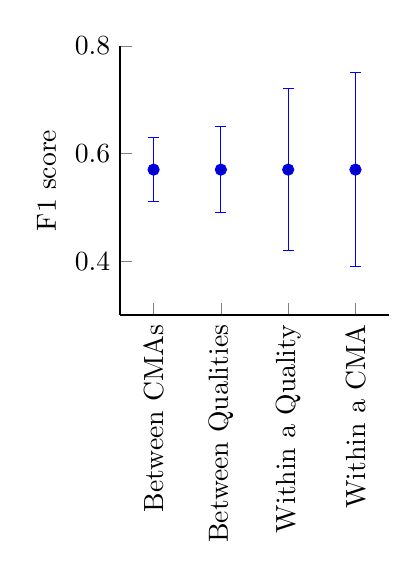
\begin{tikzpicture},
\centering
\begin{axis}[
height=5cm,
width=5cm,
ylabel={F1 score},
ymax=0.8,
ymin=0.3,
xmin=0.5,
xmax=4.5,
axis y line*=left,
axis x line*=bottom,
xticklabels={Between CMAs, Between Qualities, Within a Quality, Within a CMA},
xtick={1,2,3,4},
x tick label style={rotate=90,anchor=east}]
\addplot+[only marks][error bars/.cd,y dir=both, y explicit]
coordinates {
(1,0.57) +- (0.06,0.-0.06)
(2,0.57) +- (0.08,0.08)
(3,0.57) +- (0.15,-0.15)
(4,0.57) +- (0.18,-0.18)
};
\addplot[dashed] coordinates {(0,0) (10.5,0)};
\end{axis}
\end{tikzpicture}
\caption{Confidence intervals of F1 score in quality detection of an unseen CMA. 
Every confidence interval is two standard deviations (STD) long. 
In every trial one CMA was the test set, while the classifier was trained on the rest. The mean F1 score is 0.57. The measures from left to right are: STD between CMAs when every CMA's score is an average the scores of his or her qualities; STD between qualities when every quality's score is an average of all of the CMAs' scores for this quality; an average of qualities' STDs, where every STD is between CMAs within a quality; an average of CMAs' STDs, where every STD is between qualities within a CMA's dataset.}
\label{domainAdaptationBaseLine}
\end{figure}

\subsection{Validation on Ordinary People}
The final validation was conducted on ordinary people (non-CMAs). We
designed several daily actions (greeting friends or playing with a balloon, for
example) and the CMA committee tagged the clips. This dataset was small, with a
focus on the qualities that we found easier to recognize. The evaluation is shown in Figure \ref{nonCMAs}.

\begin{figure}[ht!]
\centering
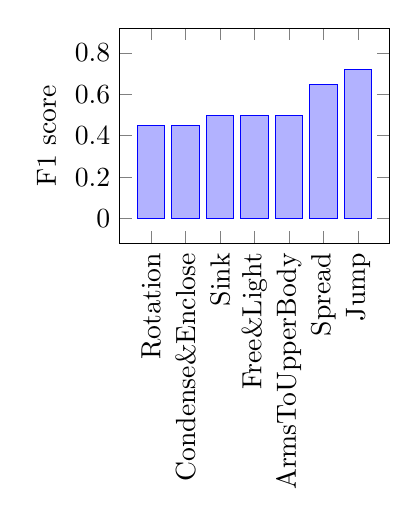
\begin{tikzpicture}
\begin{axis}[
    ymin=0,
    ymax=0.8,
    width=5cm,
    ybar stacked,
    enlargelimits=0.15,
    ylabel={F1 score},
    symbolic x coords={Rotation,Condense\&Enclose,Sink,Free\&Light,ArmsToUpperBody,Spread,Jump},
    xtick=data,
    x tick label style={rotate=90,anchor=east},
    ]
\addplot+[ybar] plot coordinates  {(Rotation,0.45) (Condense\&Enclose,0.45) (Sink,0.5) 
		(Free\&Light,0.5) (ArmsToUpperBody,0.5) (Spread, 0.65) (Jump,0.72)};

\end{axis}
\end{tikzpicture}
\caption{Performance on ordinary people (non-CMAs) instructed to
	   perform several tasks.}
\label{nonCMAs}
\end{figure}

\section{Conclusion}
We developed a method for recognizing Laban qualities using the Microsoft Kinect sensor. Our method obtained a recall and precision of about 60\% over the qualities. The larger movements, such as \textit{jump}, \textit{spread}, and \textit{sink}, are easier to quantify, and hence  easier to recognize (precision and recall of 60-90\%). The more subtle qualities, such as \textit{strong} and \textit{passive}, are harder for us to quantify in kinematic measurements, which causes a degradation in the performance (precision and recall of 40-60\%). 
\\\\The improvement of the F1 score from a single task learning setting (0.56) to a multitask setting (0.6) demonstrates the synergy of a shared model for several correlated tasks. The mild degradation of the F1 score from a seen CMA (0.6) to an unseen (0.57) shows a very good generalization ability of our linear classification model. This ability derives from our focus on the MEN regularization terms, which resulted in our model being not too rich, even sparse, and thus not over-fitted. 
\\\\Overall we believe that we succeeded in capturing the essence of most of the qualities, using a cheap (\$100) and widely available sensor.
We believe that our work will provide the foundation and inspiration that will make the LMA method
applicable in many more methodologies and processes.
\bibliographystyle{unsrt}
\bibliography{bib}
\end{document}
